\documentclass[12pt, a4paper]{article}

% Gold-Standard Academic Typography & Encoding Packages
\usepackage[T1]{fontenc}
\usepackage{lmodern}
\usepackage{microtype}
\usepackage[utf8]{inputenc}
\usepackage[margin=1in]{geometry}
\setlength{\headheight}{18pt}
\usepackage{graphicx}
\usepackage{hyperref}
\usepackage{amsmath, amssymb}
\usepackage{booktabs}
\usepackage{float}
\usepackage[export]{adjustbox}
\usepackage{listings}
\usepackage{enumitem}
\usepackage{xcolor}
\usepackage{fancyhdr}
\usepackage{array}
\usepackage{tabularx}
\usepackage{longtable}
\usepackage{caption}

% Hyperref Setup
\hypersetup{
    colorlinks=true,
    linkcolor=black,
    citecolor=black,
    urlcolor=black,
    pdftitle={Project Proposal - CampusCare},
    pdfauthor={CampusCare Development Team}
}

% Header and Footer Setup
\pagestyle{fancy}
\fancyhf{}
\rhead{\small \textbf{Software Engineering Project Proposal}}
\lhead{\small \textbf{CampusCare Proposal}}
\rfoot{\small Page \thepage}
\lfoot{\small University Infrastructure \& Facility Management}
\renewcommand{\headrulewidth}{0.4pt}
\renewcommand{\footrulewidth}{0.4pt}

\begin{document}

% =========================================================
% COVER PAGE
% =========================================================
\begin{titlepage}
    \centering
    
    % University Logo
    
\includegraphics[width=0.28\textwidth]{../srs/uits_logo.png}\\[1.2cm]
    
    {\Large \textbf{University of Information Technology and Sciences (UITS)}}\\[0.3cm]
    {\large Department of Computer Science and Engineering}\\[1.2cm]
    
    {\Large \textbf{COURSE:}} Software Project Design and Development (CSE 416)\\[1.0cm]
    
    \rule{\linewidth}{0.5mm}\\[0.4cm]
    {\LARGE \textbf{PROJECT PROPOSAL}}\\[0.2cm]
    {\large \textbf{Project Title: CampusCare}}\\[0.1cm]
    {\small Centralized University Complaint Management System}\\[0.4cm]
    \rule{\linewidth}{0.5mm}\\[1.5cm]
    
    \begin{minipage}{0.48\textwidth}
        \begin{flushleft} \large
            \textbf{Submitted To:}\\[0.2cm]
            \textbf{Al-Imtiaz}\\
            Associate Professor \& Head\\
            Ph.D. (Research Fellow), BUET\\
            Department of CSE, UITS
        \end{flushleft}
    \end{minipage}
    \hfill
    \begin{minipage}{0.48\textwidth}
        \begin{flushright} \large
            \textbf{Submitted By (Group Members):}\\[0.2cm]
            \textbf{Rudro Antony Mrong}\\
            ID: 0432320005101059\\[0.2cm]
            \textbf{Md. Masud Rahman}\\
            ID: 0432320005101064
        \end{flushright}
    \end{minipage}
    
    \vfill
    {\large Submission Date: August 2026}
\end{titlepage}

\newpage
\tableofcontents
\newpage

% =========================================================
% 1. EXECUTIVE SUMMARY
% =========================================================
\section{Executive Summary}
CampusCare is a centralized 3-tier web application designed to track, manage, and resolve university facility maintenance issues, infrastructure reporting, and operational work orders. In traditional academic institutions, complaint reporting relies on unorganized channels such as phone calls, emails, and physical front-desk logbooks. This fragmentation leads to delayed issue resolution, lost requests, lack of status tracking for reporters, and poor operational visibility for university facility managers.

CampusCare introduces a single digital workflow governed by a multi-step state machine (\texttt{Submitted}, \texttt{Assigned}, \texttt{In Progress}, \texttt{Resolved}, \texttt{Closed}, \texttt{Reopened}). The platform provides role-based web interfaces for Students, Staff, and Administrators to ensure operational accountability, track Service Level Agreement (SLA) deadlines, and provide institutional reporting on campus infrastructure maintenance.

% =========================================================
% 2. PROBLEM STATEMENT
% =========================================================
\section{Problem Statement}
Managing physical and technical infrastructure across campus lecture halls, dormitories, laboratories, and administrative offices involves thousands of active assets. Existing manual reporting workflows create several operational bottlenecks:

\begin{itemize}[leftmargin=*]
    \item \textbf{Unconsolidated Communication Channels:} Complaints submitted through emails or phone calls lead to misplaced requests and zero central record-keeping.
    \item \textbf{Lack of Reporter Status Tracking:} Students cannot track complaint progress after submission, resulting in redundant follow-up inquiries.
    \item \textbf{Unstructured Work Queues:} Maintenance staff lack prioritized digital queues, leading to uneven task distribution and missed service deadlines.
    \item \textbf{Limited Departmental Metrics:} Department heads lack quantitative data regarding active workloads, overdue tickets, resolution times, and recurring infrastructure faults.
    \item \textbf{Absence of Audit Records:} Without immutable database audit logs, tracing ticket history, verifying state changes, and evaluating historical staff performance remains difficult.
\end{itemize}

% =========================================================
% 3. PROJECT OBJECTIVES
% =========================================================
\section{Project Objectives}

\subsection{Primary Objective}
To design, develop, and deploy a responsive campus facility management platform that centralizes complaint submission, automated SLA deadline tracking, role-based dispatching, rate-limited submission APIs, and audit logging within a unified system.

\subsection{Quantifiable \& Operational Objectives}
\begin{enumerate}
    \item \textbf{Resolution Acceleration:} Reduce average complaint resolution lifecycle time across campus facility operations by 40\%.
    \item \textbf{Centralized Tracking:} Achieve 100% centralized tracking of submitted service requests through an authenticated single submission pipeline.
    \item \textbf{SLA Compliance:} Maintain institutional SLA compliance above 85\% across all complaint priority levels (\texttt{Critical: 4h}, \texttt{High: 24h}, \texttt{Medium: 72h}, \texttt{Low: 168h}).
    \item \textbf{Database Query Performance:} Maintain database response latencies below 500ms for administrative reporting queries on datasets up to 10,000 records.
    \item \textbf{Audit Traceability:} Maintain 100\% audit coverage for ticket status transitions and staff assignment updates stored in an immutable audit ledger (\texttt{audit\_logs}).
\end{enumerate}

% =========================================================
% 4. PROJECT SCOPE
% =========================================================
\section{Project Scope}

\subsection{In-Scope (Minimum Viable Product - MVP)}
The scope for the initial system release encompasses:

\begin{itemize}[leftmargin=*]
    \item \textbf{Authentication \& Security:} Email/password authentication via \texttt{@supabase/ssr}, \texttt{HttpOnly} session cookie management, Next.js Edge proxy middleware for role-based route protection (\texttt{Student}, \texttt{Staff}, \texttt{Admin}), and Upstash Redis sliding-window rate limiting (\texttt{@upstash/ratelimit}) on submission endpoints.
    \item \textbf{Student Module:} Dashboard with metric cards, complaint submission form with custom animated dropdown pickers and photo proof uploads, human-readable Complaint ID generation (\texttt{CMP-YYYY-XXXX}), real-time ticket timeline tracking, and resolution confirmation/rejection workflow.
    \item \textbf{Staff Module:} Departmental ticket queues, visual SLA deadline warning indicators, state transition controls (\texttt{Assigned} $\rightarrow$ \texttt{In Progress} $\rightarrow$ \texttt{Resolved}), internal progress note logs, manual SLA target date overrides with reason notes, and completion photo proof uploads.
    \item \textbf{Admin Module:} Global master ticket table with multi-parameter filtering using \texttt{@tanstack/react-table}, ticket reassignment and priority override controls, user role promotion and department assignment desk, category/department taxonomy management, and operational analytics charts.
    \item \textbf{Database \& Storage Infrastructure:} PostgreSQL relational schema with Row Level Security (RLS) policies utilizing \texttt{SECURITY DEFINER} helper functions to prevent policy recursion, foreign key constraints, automated ticket sequence triggers, and an immutable audit log table (\texttt{audit\_logs}).
\end{itemize}

\subsection{Out-of-Scope (Future Iterations - Version 2.0)}
The following capabilities are excluded from the initial release and reserved for future project phases:
\begin{itemize}[leftmargin=*]
    \item Automated AI complaint classification and duplicate ticket detection.
    \item Real-time WebSocket push notifications and external transactional email dispatching (e.g., Resend / SendGrid API).
    \item Native mobile applications for iOS/Android operational staff (React Native / Expo).
    \item Multi-campus organizational hierarchy support across geographically separated university branches.
\end{itemize}

% =========================================================
% 5. FEASIBILITY STUDY
% =========================================================
\section{Feasibility Study}

\subsection{Technical Feasibility}
The system leverages Next.js 16 (App Router), React 19, TypeScript, Tailwind CSS, \texttt{@tanstack/react-table}, and Supabase (PostgreSQL). This stack provides standard SSR support, strong type safety, and clean separation of client and server logic. Supabase Row Level Security (RLS) combined with \texttt{SECURITY DEFINER} SQL helper functions enforces strict role-based data isolation at the database layer. Upstash Redis handles request rate limiting to protect public endpoints against abuse.

\subsection{Operational Feasibility}
The UI is built using the Caring Campus Green design system with responsive layouts supporting viewports down to 320px width and high-contrast text meeting WCAG standards. The system reflects standard university facility workflows (\texttt{Student reports} $\rightarrow$ \texttt{System/Admin assigns} $\rightarrow$ \texttt{Staff resolves} $\rightarrow$ \texttt{Student verifies}), requiring minimal training for campus maintenance personnel and students.

\subsection{Economic Feasibility}
Next.js, React, Tailwind CSS, and PostgreSQL incur zero software licensing fees. Hosting on Vercel and Supabase keeps operational overhead low, starting on free dev tiers and scaling to modest Pro tiers (\$45/month total) for production workloads, significantly reducing manual administrative labor costs.

% =========================================================
% 6. TARGET AUDIENCE & ROLE MATRIX
% =========================================================
\section{Target Audience \& Role Capability Matrix}

\begin{table}[H]
\centering
\small
\begin{tabularx}{\textwidth}{X c c c}
\toprule
\textbf{Capability / Function} & \textbf{Student Role} & \textbf{Staff Role} & \textbf{Admin Role} \\
\midrule
Submit New Complaint & Yes & No & No \\
View Personal Submitted Complaints & Yes & No & Yes (All) \\
View Department Assigned Complaints & No & Yes & Yes (All) \\
Claim / Accept Ticket \& Update Status & No & Yes & Yes \\
Override Ticket Priority \& SLA Target & No & Yes & Yes \\
Append Progress Notes & Public Notes Only & Yes & Yes \\
Confirm or Reject Resolution & Yes & No & Yes (Override) \\
Assign or Reassign Staff/Department & No & No & Yes \\
Promote User \& Assign Staff Department & No & No & Yes \\
View System Audit Logs & No & No & Yes (Read-Only) \\
\bottomrule
\end{tabularx}
\caption{Role Capability Matrix across CampusCare User Roles.}
\end{table}

% =========================================================
% 7. WORK BREAKDOWN STRUCTURE (WBS)
% =========================================================
\section{Work Breakdown Structure (WBS) \& Task Costing}

\begin{figure}[H]
    \centering
    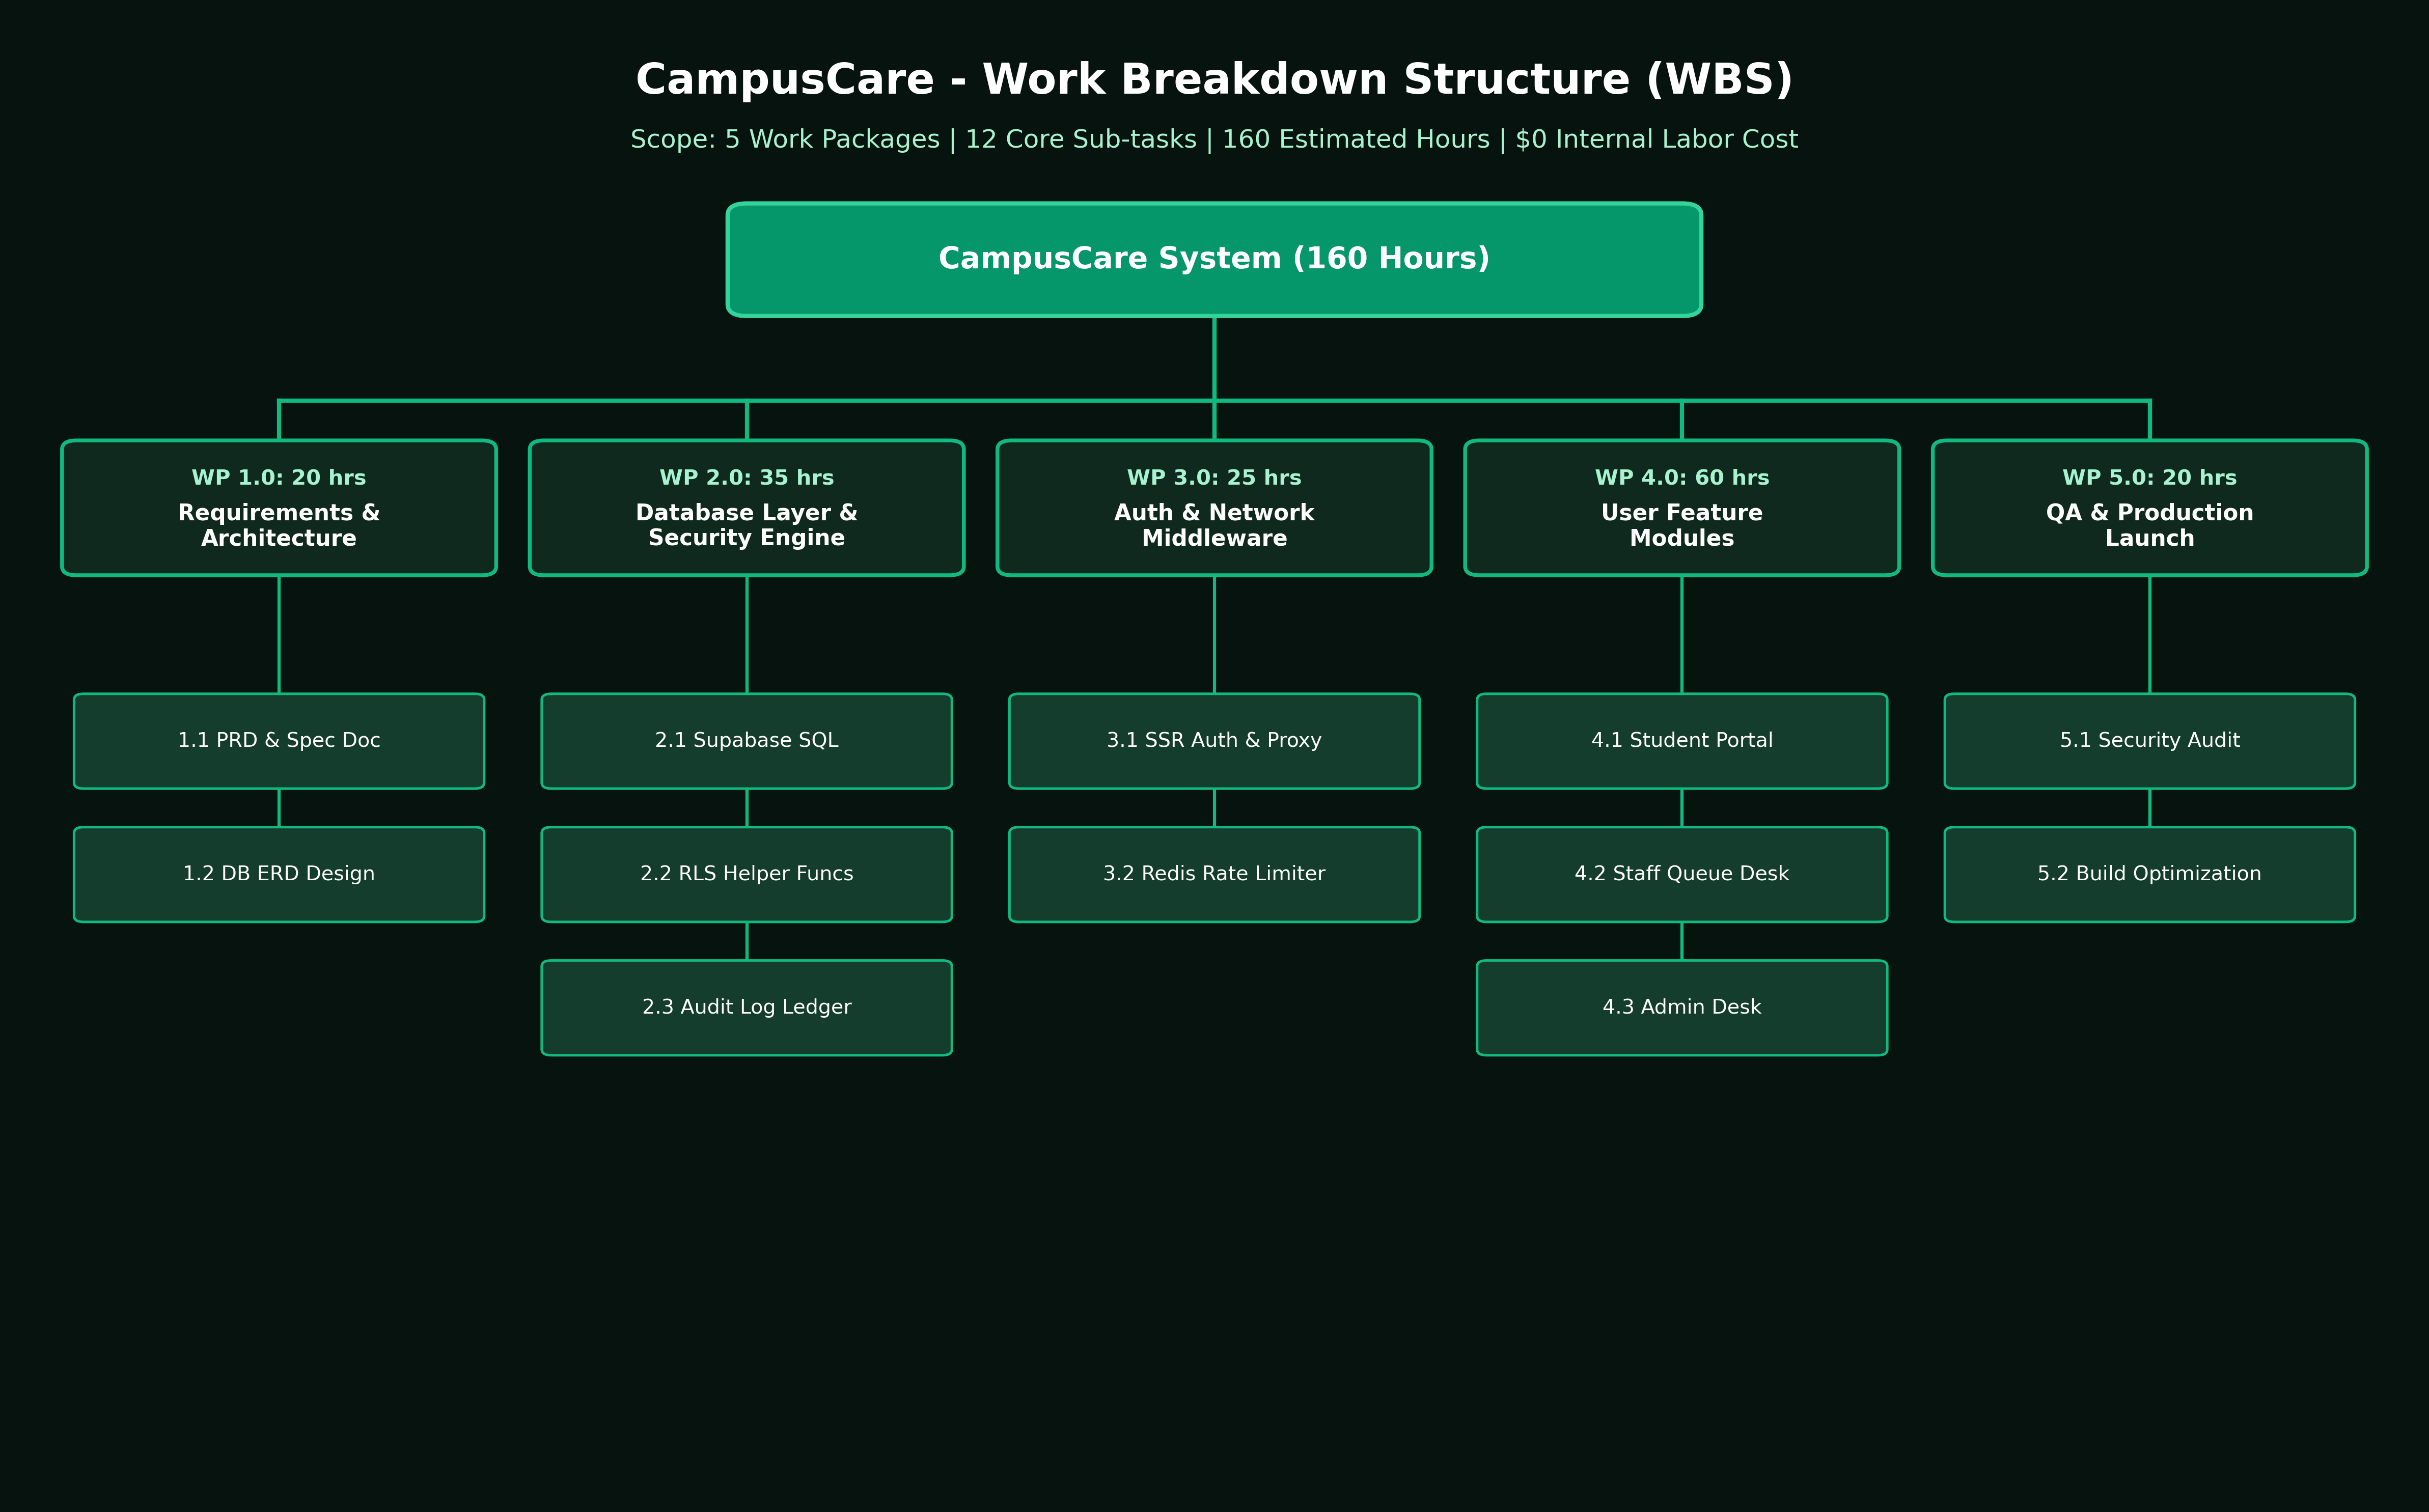
\includegraphics[width=0.95\textwidth]{../diagrams/campuscare_wbs.png}
    \caption{CampusCare Work Breakdown Structure (WBS) Tree Diagram.}
    \label{fig:wbs}
\end{figure}

\begin{table}[H]
\centering
\small
\begin{tabularx}{\textwidth}{l X c c}
\toprule
\textbf{Work Package} & \textbf{Title \& Deliverables} & \textbf{Labor (Hours)} & \textbf{Cost (USD)} \\
\midrule
\textbf{WP 1.0} & Requirements \& Architecture (PRD, Spec, ERD) & 20 hrs & \$0.00 \\
\textbf{WP 2.0} & Database \& Security (PostgreSQL, RLS, Audit Log) & 35 hrs & \$0.00 \\
\textbf{WP 3.0} & Auth \& Middleware (\texttt{@supabase/ssr}, Proxy, Redis) & 25 hrs & \$0.00 \\
\textbf{WP 4.0} & Core Modules (Student, Staff, Admin Desks) & 60 hrs & \$0.00 \\
\textbf{WP 5.0} & QA \& Launch (Security Audit, WCAG, Build Optimization) & 20 hrs & \$0.00 \\
\midrule
\textbf{Total Project} & \textbf{5 Work Packages (12 Sub-tasks)} & \textbf{160 Hours} & \textbf{\$0.00} \\
\bottomrule
\end{tabularx}
\caption{Work Package Task \& Labor Costing Breakdown.}
\end{table}

% =========================================================
% 8. PROJECT TIMELINE & GANTT CHART
% =========================================================
\section{Project Timeline \& Gantt Chart}

\begin{figure}[H]
    \centering
    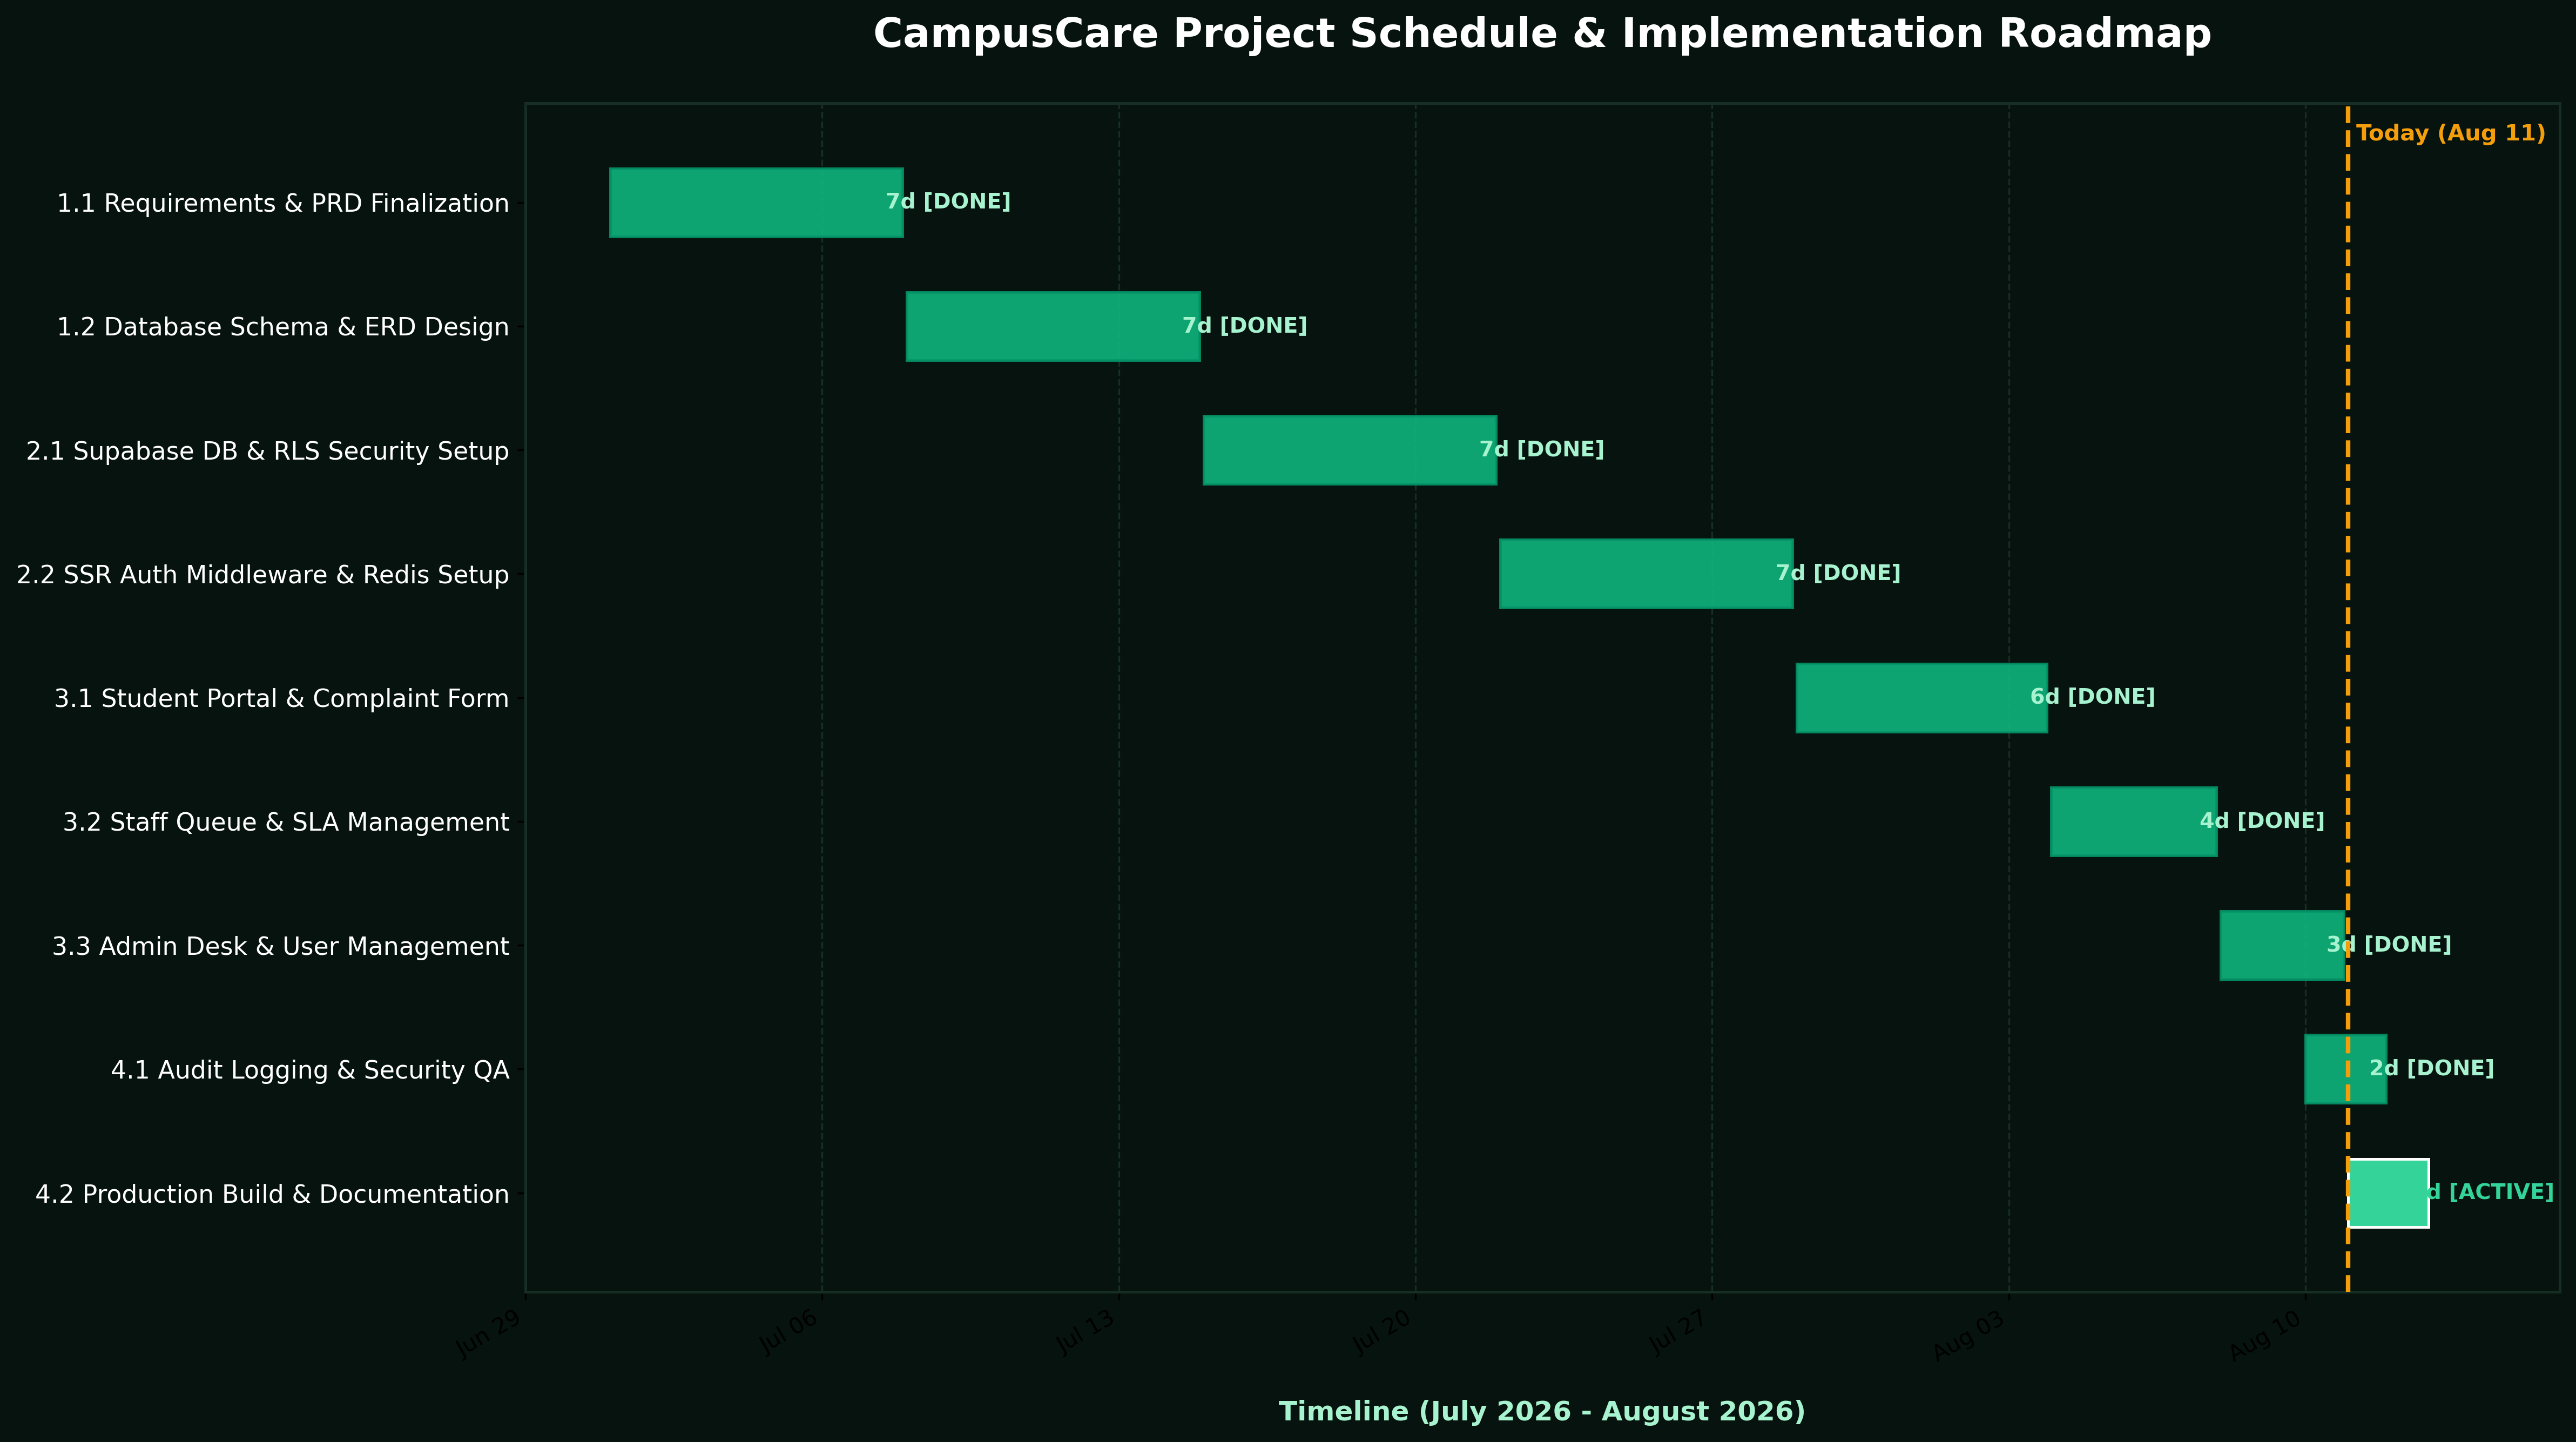
\includegraphics[width=0.95\textwidth]{../diagrams/campuscare_gantt.png}
    \caption{CampusCare Project Implementation Schedule \& Roadmap.}
    \label{fig:gantt}
\end{figure}

% =========================================================
% 9. BUDGET & COST ESTIMATION
% =========================================================
\section{Budget \& Cost Estimation}

\begin{table}[H]
\centering
\small
\begin{tabularx}{\textwidth}{p{0.24\textwidth} X c r}
\toprule
\textbf{Category} & \textbf{Component / Resource} & \textbf{Quantity} & \textbf{Annual Cost (USD)} \\
\midrule
Development & Internal Engineering Team & 1 Team & \$0.00 \\
Application Hosting & Vercel Hosting (Pro Tier) & 12 Months & \$240.00 \\
Database \& Auth & Supabase Managed PostgreSQL (Pro Tier) & 12 Months & \$300.00 \\
Rate Limiting & Upstash Redis Cloud & 12 Months & \$120.00 \\
Domain \& Network & Campus Subdomain (\texttt{campuscare.}\\ \texttt{university.edu}) & 1 Domain & \$0.00 \\
SSL Certificate & Vercel / Let's Encrypt Automated SSL & 1 Certificate & \$0.00 \\
Buffer / Storage & Bandwidth \& Storage Contingency Buffer & 1 & \$100.00 \\
\midrule
\multicolumn{3}{l}{\textbf{Total Annual Cost}} & \textbf{\$760.00} \\
\bottomrule
\end{tabularx}
\caption{Annualized Cloud Infrastructure \& Operational Budget Breakdown.}
\end{table}

% =========================================================
% 10. SYSTEM ARCHITECTURE & TECHNICAL STACK
% =========================================================
\section{System Architecture \& Technical Stack}

\begin{itemize}[leftmargin=*]
    \item \textbf{Presentation Layer (Frontend):} Built using Next.js 16 (App Router), React 19, TypeScript, styled with Tailwind CSS using the Caring Campus Green design system. Data tables utilize \texttt{@tanstack/react-table}. Responsive layouts support mobile viewports down to 320px width.
    \item \textbf{Application Layer (Backend):} Server-side logic and API routes managed in Next.js. Server validation handled by Zod schemas. Session handling managed via \texttt{@supabase/ssr} with Edge proxy middleware. API protection handled by Upstash Redis sliding-window rate limiters.
    \item \textbf{Data \& Storage Layer:} Relational database on Supabase PostgreSQL. Row Level Security (RLS) policies enforced at the database engine level. Uploaded attachments stored in Supabase Storage buckets with MIME-type validation.
\end{itemize}

% =========================================================
% 11. SUCCESS METRICS & EVALUATION CRITERIA
% =========================================================
\section{Success Metrics \& Evaluation Criteria}

\begin{itemize}[leftmargin=*]
    \item \textbf{Resolution Speed:} Achieving at least a 90\% completion rate for submitted complaints reaching \texttt{Closed} status within target SLA limits.
    \item \textbf{SLA Compliance:} Maintaining $>85\%$ compliance with target resolution timeframes across all priority levels.
    \item \textbf{Query Performance:} Maintaining administrative master table query response times under 500ms for datasets up to 10,000 complaint records.
    \item \textbf{User Feedback:} Achieving an average user satisfaction rating of at least 4.0 out of 5.0 stars on closed ticket evaluations.
\end{itemize}

\end{document}
